
\section{Proofs of formal statements}

\subsection{Proposition~\refmain{prop:optimal-convergence} -- optimal convergence}

\begin{propositionmain}{\refmain{prop:optimal-convergence}}
	Let us consider MDPs $\Model_0, \dots, \Model_{n}$ and their associated mapping functions $\Mapping_0, \dots, \Mapping_{n-1}$.
	If $\RlAlgo$ is an off-policy learning algorithm, then,
	in every $i$-th iteration of Algorithm~\refmain{alg:main}, $\Est{\Policy}^*_i$ converges to $\Policy^*_i$,
	as the number of environment interactions increase.
\end{propositionmain}
\begin{proof}
	At any iteration $i \in \{n, \dots, 0\}$ of Algorithm~\refmain{alg:main},
	we are given $\Model_i$, $\Mapping_i$ and~$\Est{V}_{i+1}^*$.
	By construction, the two instantiations of $\RlAlgo$, $\DLearner_i$ and $\Biased{\DLearner}_i$,
	perform updates from transitions generated from $\Model_i$ and $\Biased{\Model}_i$, respectively.
	Actions are selected according to $\Biased{\DLearner}_i$ which follows some exploration policy $\Biased\ExplorationPolicy$.
	Since $\Model_i$ and $\Biased{\Model}_i$ share the same state and action spaces,
	$\Biased\ExplorationPolicy$ is also an exploration policy for~$\Model_i$, in the sense of Definition~\refmain{def:off-policy-learning}.
	Therefore, ${\DLearner}_i$ also converges to $\Policy^*_i$, as the number of environment interactions $t \to \infty$.
\end{proof}


\subsection{Lemma~\refmain{lem:multi-step} -- multi-step value}

\begin{lemmamain}{\refmain{lem:multi-step}}
	Given a goal MDP $\Model$ and $\Mapping: \States \to \Abst\States$,
	for any $s \in \States$ and $\Mapping$-relative option~$o$, the optimal value of~$o$ is:
	\begin{equation}
		Q^*(s, o) =
			\sum_{k=0}^{\infty} \gamma^k \sum_{s_{1:k} \in \Mapping(s)^k} \sum_{s' \not\in \Mapping(s)}
			p(s_{1:k} s' \Given s, \Policy_o)\, \bigl( \Indicator(s' \in \Goals) + \gamma\, V^*(s') \bigr)
	\end{equation}
\end{lemmamain}
\begin{proof}
	By assumption $\Model$ is a goal MDP over some $\Goals \subseteq \States$.
	For $s \in \Goals$, we know $Q^*(s, o) = 0$. We consider $s \not\in \Goals$.
	Since the MDP $\Model$ is clear from the context, to uniform the notation, we use $p(s' \Given s, a)$ instead of $T(s, a, s')$.
	Following a similar procedure as~\cite{abel_2020_ValuePreserving}, for our definition of goal MDPs:
	\begin{align}
		{Q}^*(s, o) &\!\coloneqq 
			\Expected_{s' \Given s, o}[\, R(s, \Policy_o(s), s')\, +
				\gamma (\, \Indicator(s' \in \Mapping(s))\, {Q}^*(s', o)
				+ \Indicator(s' \not\in \Mapping(s))\, {V}^*(s'))\,] \\
			&= \sum_{s' \in \Mapping(s)} p(s' \Given s, \Policy_o(s))[\,\cdot\,] +
				\sum_{s' \not\in \Mapping(s)} p(s' \Given s, \Policy_o(s))[\,\cdot\,] \\
			&= \sum_{s' \in \Mapping(s)} p(s' \Given s, \Policy_o(s)) \,
					\gamma \, {Q}^*(s', o)\, +
				\sum_{s' \not\in \Mapping(s)} p(s' \Given s, \Policy_o(s)) \bigl(
					\Indicator(s' \in \Goals) + \gamma\, {V}^*(s')
				\bigr) 
				\label{eq:option-value-to-expand}
	\end{align}
	We abbreviate the second term of~\eqrefthis{eq:option-value-to-expand} with $\Psi$ and let $s_0 = s$.
	Then, similarly to the classic multi-step value of options~\cite{sutton1999between}, we can expand over time.
	\begin{align}
		&Q^*(s, o) = \sum_{s' \in \Mapping(s)} p(s' \Given s, \Policy_o(s)) \,
					\gamma \, {Q}^*(s', o)\, + \Psi(s, o)\\
			&= \Psi(s, o) + \gamma\, \sum_{s' \in \Mapping(s)} p(s' \Given s,
					\Policy_o(s))\,\Psi(s', o) \,+
				\gamma^2 \sum_{s', s'' \in \Mapping(s)^2} 
				p(s'\,s'' \Given s, \Policy_o(s)\,\Policy_o(s'))\, Q^*(s'', o)\\
			&= \sum_{k=0}^{\infty} \gamma^k\, \sum_{s_{1:k} \in \Mapping(s)^{k}}
				p(s_{1:k} \Given s, \Policy_o)\,\Psi(s_{k}, o)\\
			&= \sum_{k=0}^{\infty} \gamma^k\,
				\sum_{s_{1:k} \in \Mapping(s)^k} \sum_{s'\not\in \Mapping(s)}
				p(s_{1:k} s' \Given s, \Policy_o)\, \bigl(
				\Indicator(s' \in \Goals) + \gamma\, V^*(s') \bigr)
				\label{eq:options-multistep-proof-end}
	\end{align}
	which is the expression in Lemma~\refmain{lem:multi-step}.
\end{proof}

With a similar procedure, we can also show that the multi-step value of a $\Mapping$-relative
option~$o$ in a biased MDP $\Biased\Model$ with respect to $\langle \Abst\Model, \Mapping \rangle$ is:
\begin{align}
	\BiasedStar{Q}(s, o)
		&= \sum_{k=0}^{\infty} \gamma^k\,
			\sum_{s_{1:k} \in \Mapping(s)^k} \sum_{s' \not\in \Mapping(s)}
			p(s_{1:k} s' \Given s, \Policy_o) \, \bigl(
		\Indicator(s' \in \Goals) + \gamma\, \Abst{V}^*(\Mapping(s'))
			- \Abst{V}^*(\Mapping(s)) + \gamma\, V^*(s') \bigr)
\end{align}


\subsection{Lemma~\refmain{lem:marginalized-optq} -- marginalized value}
\begin{lemmamain}{\refmain{lem:marginalized-optq}}
	Let $\Model$ be an MDP and $\langle \Abst{\Model}, \Mapping \rangle$ its abstraction, satisfying assumptions~\refmain{as:goal} and \refmain{as:abstract-goal}.
	The value of any $\Mapping$-relative option~$o$ in~$\Model$ admits the following lower bound:
	\begin{equation}
		Q^*(s, o) \ge
			\sum_{\Abst{s}' \in \Abst\States \setminus \{\Mapping(s)\}} \sum_{k=0}^{\infty}
					\gamma^k\, p(\FromBlockTo{s}{k}{\Abst{s}'} \Given s, \Policy_{o})\,
					\bigl(
			\Indicator(\Abst{s}' \in \Abst{\Goals}) + \gamma\, (W_\PHomogeneity(\Mapping(s), \Abst{s}') - \PHomogeneity) \bigr)
	\end{equation}
	at any $s \in \States$, where,~$\PHomogeneity$ and~$W_\PHomogeneity$\, follow Definition~\refmain{def:equipotentials}.
\end{lemmamain}
\begin{proof}
	We recall that $p(\FromBlockTo{s}{k}{\Abst{s}'} \Given s, \Policy)$ denotes
	the probability of the event of remaining for~$k$ steps within
	$\Mapping(s)$, then reaching~$\Abst{s}'$ at the next transition, when following policy~$\Policy$, starting from~$s$.
	Similarly, we use $p(\FromBlockTo{s}{k}{{s}'} \Given s, \Policy)$ to represent
	the probability of remaining $k$~steps within $\Mapping(s)$ then reaching a specific ground state $s' \in \States \setminus \Mapping(s)$.

	To obtain the result, we marginalize the probabilities appearing in
	Lemma~\refmain{lem:multi-step} over all possible trajectories~$s_{1:k}$:
	\begin{align}
		Q^*(s, o) &= \sum_{s' \in \States \setminus \Mapping(s)} \sum_{k=0}^{\infty}
					\gamma^k\, p(\FromBlockTo{s}{k}{s'} \Given s, \Policy_{o})\, \bigl(
			\Indicator(s' \in \Goals) + \gamma\, V^*(s') \bigr)
		\label{eq:marginalized-ground-value}
	\end{align}
	Now, for all $s', k$ such that $p(\FromBlockTo{s}{k}{s'} \Given s, \Policy_{o}) > 0$,
	there is one state $s_k \in \Mapping(s)$, reachable in $k$ steps from~$s$ under~$\Policy_o$, from which $T(s_k, \Policy_o(s_k), s') > 0$.
	From Definition~\refmain{def:equipotentials}, we know $\abs{W_\PHomogeneity(\Mapping(s_k), \Mapping(s')) - V^*(s')} \le \PHomogeneity$.
	Therefore, we can provide a lower bound for each term $V^*(s')$ in the sum above:
	\begin{equation}
		Q^*(s, o) \ge \sum_{s' \in \States \setminus \Mapping(s)} \sum_{k=0}^{\infty}
					\gamma^k\, p(\FromBlockTo{s}{k}{s'} \Given s, \Policy_{o})\, \bigl(
			\Indicator(s' \in \Goals) + \gamma\, (W_\PHomogeneity(\Mapping(s), \Mapping(s')) - \PHomogeneity) \bigr)
	\end{equation}
	because $\Mapping(s_k) = \Mapping(s)$.
	It is now possible to split the sum $\sum_{s' \in \States \setminus \Mapping(s)}$ into
	${\abs{\Abst{\States}} - 1}$ sums over future blocks and marginalize among them to obtain:
	\begin{equation}
			Q^*(s, o) \ge
				\sum_{\Abst{s}' \in \Abst\States \setminus \{\Mapping(s)\}} \sum_{k=0}^{\infty}
						\gamma^k\, p(\FromBlockTo{s}{k}{\Abst{s}'} \Given s, \Policy_{o})\,
						\bigl(
				\Indicator(\Abst{s}' \in \Abst\Goals) + \gamma\, (W_\PHomogeneity(\Mapping(s), \Abst{s}') - \PHomogeneity) \bigr)
	\end{equation}
	since $\Indicator(s \in \Goals) = \Indicator(\Mapping(s) \in \Abst\Goals)$.
	This proves the lemma. With the same procedure, we also obtain the upper bound:
	\begin{equation}
			Q^*(s, o) \le
				\sum_{\Abst{s}' \in \Abst\States \setminus \{\Mapping(s)\}} \sum_{k=0}^{\infty}
						\gamma^k\, p(\FromBlockTo{s}{k}{\Abst{s}'} \Given s, \Policy_{o})\,
						\bigl(
				\Indicator(\Abst{s}' \in \Abst\Goals) + \gamma\, (W_\PHomogeneity(\Mapping(s), \Abst{s}') + \PHomogeneity) \bigr)
	\end{equation}
\end{proof}


\subsection{Theorem~\refmain{th:exploration-loss-bound} -- exploration loss}

\begin{theoremmain}{\refmain{th:exploration-loss-bound}}
	Let $\Model$ and $\langle \Abst\Model, \Mapping \rangle$ be and MDP and an abstraction satisfying assumptions~\refmain{as:goal} and \refmain{as:abstract-goal},
	and let $\Biased\Model$ be the biased MDP.
	If $\epsilon$ is the abstract similarity of $\Policy^*$ and $\BiasedStar{\Policy}$, and the abstract value approximation is~$\PHomogeneity$, then, the exploration loss of $\langle \Abst\Model, \Mapping \rangle$ satisfies:
	\begin{equation}
		L(\Model, \langle \Abst\Model, \Mapping \rangle) \le
			\frac{2 \abs{\Abst\States} (\POptAccurate + \gamma\, \PHomogeneity)}{(1-\gamma)^2}
	\end{equation}
\end{theoremmain}
\begin{proof}
	Any policy $\Policy$ can be represented as a set $\Options$, composed of $\Mapping$-relative options
	whose initiation sets are partitioned according to $\Mapping$ and $\forall s \in \States,
	\exists o \in \Options: {\Policy_o(s) = \Policy(s)}$.
	Let $\Options^*$ and $\BiasedStar\Options$ be the $\Mapping$-relative options associated to $\Policy^*$ and $\BiasedStar\Policy$.
	We now compute what is the difference in value between executing $\Policy^*$ and $\BiasedStar\Policy$,
	for one option each, then following $\Policy^*$ afterwards.
	For any $s \in \States \setminus \Goals$, let $o^*$ and $\BiasedStar{o}$ be the relevant options in $\Options^*$ and $\BiasedStar{O}$, respectively.
	We bound the following difference in value:
	\begin{align}
			\abs{Q^*(s, o^*) - Q^*(s, \BiasedStar{o})} =
			Q^*(s, o^*) - Q^*(s, \BiasedStar{o})
	\end{align}
	From an application of the upper and lower bound of Lemma~\refmain{lem:marginalized-optq},
	\begin{align}
		&\abs{Q^*(s, o^*) - Q^*(s, \BiasedStar{o})} \\
			&\le \sum_{\Abst{s}' \in \Abst\States \setminus \{\Mapping(s)\}} \sum_{k=0}^{\infty}
						\gamma^k\, p(\FromBlockTo{s}{k}{\Abst{s}'} \Given s, \Policy_{o^*})\,
						\bigl(
				\Indicator(\Abst{s}' \in \Abst\Goals) + \gamma\, (W_\PHomogeneity(\Mapping(s), \Abst{s}') + \PHomogeneity) \bigr)\, - \notag\\
			&\qquad\sum_{\Abst{s}' \in \Abst\States \setminus \{\Mapping(s)\}} \sum_{k=0}^{\infty}
						\gamma^k\, p(\FromBlockTo{s}{k}{\Abst{s}'} \Given s, \Policy_{\BiasedStar{o}})\,
						\bigl( \Indicator(\Abst{s}' \in \Abst\Goals) + \gamma\, (W_\PHomogeneity(\Mapping(s), \Abst{s}') - \PHomogeneity) \bigr)\\
			&=\sum_{\Abst{s}' \in \Abst\States \setminus \{\Mapping(s)\}}
						\bigl( \Indicator(\Abst{s}' \in \Abst\Goals) + \gamma\, W_\PHomogeneity(\Mapping(s), \Abst{s}') \bigr)
						\sum_{k=0}^{\infty}
						\gamma^k\, \bigl(\, p(\FromBlockTo{s}{k}{\Abst{s}'} \Given s, \Policy_{o^*}) - p(\FromBlockTo{s}{k}{\Abst{s}'} \Given s, \Policy_{\BiasedStar{o}}) \bigr)\, + \notag\\
			&\qquad\sum_{\Abst{s}' \in \Abst\States \setminus \{\Mapping(s)\}} \sum_{k=0}^{\infty}
						\gamma^k\, \bigl(\, p(\FromBlockTo{s}{k}{\Abst{s}'} \Given s, \Policy_{o^*}) + p(\FromBlockTo{s}{k}{\Abst{s}'} \Given s, \Policy_{\BiasedStar{o}}) \bigr)
						\, \gamma\, \PHomogeneity
	\end{align}
	Now we apply Definition~\refmain{def:similar-policies} of abstract similarity and bound
	\begin{align}
		\abs{Q^*(s, o^*) \,&-\, Q^*(s, \BiasedStar{o})} \\
			&\le \sum_{\Abst{s}' \in \Abst\States \setminus \{\Mapping(s)\}}
					\bigl( \Indicator(\Abst{s}' \in \Abst\Goals) + \gamma\, W_\PHomogeneity(\Mapping(s), \Abst{s}') \bigr)
			\sum_{k=0}^{\infty}
						\gamma^k\, \POptAccurate\, +
			\sum_{\Abst{s}' \in \Abst\States \setminus \{\Mapping(s)\}} \sum_{k=0}^{\infty}
						\gamma^{k+1}\, 2 \, \PHomogeneity\\
			&= \sum_{\Abst{s}' \in \Abst\States \setminus \{\Mapping(s)\}}
					\Bigl(\bigl( \Indicator(\Abst{s}' \in \Abst\Goals) + \gamma\, W_\PHomogeneity(\Mapping(s), \Abst{s}') \bigr)
					\frac{\POptAccurate}{1-\gamma} +
					\frac{2\, \gamma\, \PHomogeneity}{1-\gamma} \Bigr)
	\end{align}
	Since in a goal MDP the maximum value is 1, we know 
	$W_\PHomogeneity(\Mapping(s), \Abst{s}') \le (1 + \PHomogeneity)$, for all $s \in \States, \Abst{s}' \in \Abst\States$.
	Moreover, if $W_\PHomogeneity$ satisfies condition \eqrefmain{eq:equipotentials},
	the function $W_{\PHomogeneity}^{\text{clip}}(\Abst{s}, \Abst{s}') \coloneqq \min\{1, W_\PHomogeneity(\Abst{s}, \Abst{s}')\}$
	also satisfies it. Concluding,
	\begin{align}
			\abs{Q^*(s, o^*) - Q^*(s, \BiasedStar{o})}
			&\le \sum_{\Abst{s}' \in \Abst\States \setminus \{\Mapping(s)\}}
					\Bigl(\bigl( 1 + \gamma \bigr)
					\frac{\POptAccurate}{1-\gamma} +
					\frac{2\, \gamma\, \PHomogeneity}{1-\gamma} \Bigr)\\
			&\le \abs{\Abst\States}
					\Bigl(
					\frac{2\, \POptAccurate}{1-\gamma} +
					\frac{2\, \gamma\, \PHomogeneity}{1-\gamma} \Bigr)\\
			&= \frac{2 \abs{\Abst\States} (\POptAccurate + \gamma\, \PHomogeneity)}{1-\gamma}
	\end{align}
	This is a bound on the value loss of executing a single option from the set $\BiasedStar\Options$.
	To this option set the results from \cite{abel_2020_ValuePreserving} apply and equation~(3), in particular.
	So we obtain the final result:
	\begin{equation}
		L(\Model, \langle \Abst\Model, \Mapping \rangle) \le
			\frac{2 \abs{\Abst\States} (\POptAccurate + \gamma\, \PHomogeneity)}{(1-\gamma)^2}
	\end{equation}
\end{proof}


\section{Experimental details}


\subsection{Details for each plot}

In this section, we provide details and hyper-parameters for each plot of the main paper.
An even more comprehensive list can be found in the subdirectories of the archive \verb|experiments.tar.bz2|,
that is distributed together within the software repository\footnote{\texttt{https://github.com/cipollone/multinav2}},
at release \verb|v0.2.7|.
The structure of this archive will be discussed in section~\refthis{sec:using}.

\subsubsection*{Figure~\refmain{fig:4rooms-steps}}
\paragraph{Environment}
The ground environment, $\Model_1$, is the 4-rooms map appearing in~\cite{sutton1999between,abel_2020_ValuePreserving}.
Transitions have 4\% failure probability (another random action is executed instead).
The agent starts in the lower-left room, coordinate $(1, 9)$ (vertical coordinate increases downward).
Episode maximum length 50 steps, discounting $\gamma_1 = 0.98$.
The abstraction, $\Model_2$, is a 4-states environment with 10\% failure probability, discounting $\gamma_2 = 0.9$.

\paragraph{Algorithms}
Each point in the plot shows average and standard deviation computed over evaluations of 10 different runs.
Each evaluation computes the average episode length (time to goal or to timeout) from 10 episodes.
\begin{itemize}
	\item DelayedQ algorithm,
		$\epsilon_1 = 0.01$, $\delta = 0.1$, $\text{MaxR} = 1.0$, $m = 15$,
		60000 timesteps.
	\item Q-learning,
		learning rate decay from 0.1 to 0.02, 
		$\epsilon$-greedy exploration decay from 1.0 to 0.0.
		60000 timesteps.
	\item Q-learning with our Reward Shaping,
		learning rate decay from 0.1 to 0.02,
		$\epsilon$-greedy exploration decay from 1.0 to 0.0.
		50000 timesteps.
		The plot shows the performance of~$\Est{\Policy}_1^*$.
\end{itemize}


\subsubsection*{Figure~\refmain{fig:8rooms-steps}}
\paragraph{Environment}
The ground environment, $\Model_1$, is the 8-rooms map of Figure~\refmain{fig:rooms8}.
Transitions have 4\% failure probability.
The agent starts in the upper-left room, coordinate $(2, 3)$.
Episode maximum length 70 steps, discounting $\gamma_1 = 0.98$.
The abstraction, $\Model_2$, is a 8-states environment with 10\% failure probability, discounting $\gamma_2 = 0.9$.

\paragraph{Algorithms}
Each point in the plot shows average and standard deviation computed over evaluations of 10 different runs.
Each evaluation computes the average episode length from 10 episodes.
\begin{itemize}
	\item DelayedQ algorithm,
		$\epsilon_1 = 0.005$, $\delta = 0.1$, $\text{MaxR} = 1.0$, $m = 15$,
		300000 timesteps.
	\item Q-learning,
		learning rate decay from 0.05 to 0.01, 
		$\epsilon$-greedy exploration decay from 1.0 to 0.1.
		300000 timesteps.
	\item Q-learning with our Reward Shaping,
		learning rate decay from 0.05 to 0.01,
		$\epsilon$-greedy exploration decay from 1.0 to 0.1.
		290000 timesteps.
		The plot shows the performance of~$\Est{\Policy}_1^*$.
\end{itemize}


\subsubsection*{Figure~\refmain{fig:8rooms-inv}}
\paragraph{Environment}
Same environment as in Figure~\refmain{fig:8rooms-steps}.

\paragraph{Algorithms}
Each point in the plot shows average and standard deviation computed over evaluations of 10 different runs.
Each evaluation computes the average episode length from 10 episodes.
The plots show the performance of~$\Est{\Policy}_1^*$.
\begin{itemize}
	\item Q-learning with our Reward Shaping,
		learning rate decay from 0.05 to 0.01,
		$\epsilon$-greedy exploration decay from 1.0 to 0.1.
		290000 timesteps.
	\item Q-learning with the same potential we use in our Reward Shaping,
		with the only difference the potential is zero when the episode ends.
		Learning rate decay from 0.05 to 0.01,
		$\epsilon$-greedy exploration decay from 1.0 to 0.1.
		290000 timesteps.
\end{itemize}


\subsubsection*{Figure~\refmain{fig:reach-abs-errors}}
\paragraph{Environment}
Same environment as in Figure~\refmain{fig:8rooms-steps}.

\paragraph{Algorithms}
Each point in the plot shows average and standard deviation computed over evaluations of 10 different runs.
Each evaluation computes the average episode length from 10 episodes.
The three agents are trained with the same parameters:
\begin{itemize}
	\item Q-learning with our Reward Shaping,
		learning rate decay from 0.05 to 0.01,
		$\epsilon$-greedy exploration decay from 1.0 to 0.1.
		400000 timesteps.
		The plot shows the performance of~$\Est{\Policy}_1^*$.
\end{itemize}
The only difference between the three executions is in the potential induced by the abstract MDP $\Model_2$.
This is described in the main paper.


\subsubsection*{Figure~\refmain{fig:task-cont-dqn}}
\paragraph{Environment}

\begin{figure}
	\centering
	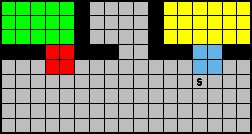
\includegraphics{./imgs/office-grid.pdf}
	\caption{Map used for the plots in Figure~\refmain{fig:task-cont-dqn}.}
	\label{fig:office-map}
\end{figure}
In the most abstract environment, $\Model_{2,d}$,
each state represents a color of Figure~\refthis{fig:office-map}.
A transition is possible if two colors are adjacent in the map. 
Failure probability 10\% and discounting $\gamma_2 = 0.9$.
States of the lower model, $\Model_{1,d}$, represent the cells of Figure~\refthis{fig:office-map}. 
Failure probability 4\% and discounting $\gamma_1 = 0.98$.
In the ground dynamics, $\Model_{0,d}$, the agent moves with continuous increments over the same map.
Specifically, the actions are $\Actions_0 = \{ \Const{Left}, \Const{Right}, \Const{Accelerate}, \Const{Decelerate}, \Const{Interact}, \Const{NoOp} \}$.
$\Const{Left}$ and $\Const{Right}$ actions rotate the agent base by increments of 40°.
$\Const{Accelerate}$ and $\Const{Decelerate}$ increase and decrease linear velocity by 0.2 cells per step.
Maximum and minimum velocity are 0.6 and 0.0 cells per step.
The states are composed of $(x, y, \cos(\theta), \sin(\theta), v \cos(\theta), v \sin(\theta)) \in \States_0$.
Failure probability 3\%, episode maximum length 200, discounting $\gamma_0 = 0.99$.
Each model dynamics is $\Model_{i,d}$ is then composed with the automaton
of Figure~\refmain{fig:office-automa} to obtain a goal MDP~$\Model_i$.
Training is performed over each $\Model_i$. Further references are provided in the main paper.
The mapping $\Mapping_1$ preserves the current color and automaton state.
The mapping $\Mapping_0$ preserves the current cell and automaton state.
Note that, unlike in the 8-rooms map, the different regions touch in more than one location.


\paragraph{Algorithms}
Each point in the plot shows average and standard deviation computed over evaluations of 5 different runs.
Each evaluation computes the average episode length from 2 episodes.
\begin{itemize}
	\item Dueling DQN,
		learning rate 0.0005, 
		$\epsilon$-greedy exploration decay from 0.85 to 0.05,
		replay buffer of 80000 transitions,
		train batch size 64, 4 optimization per environment step,
		target network update frequency 1000 steps,
		840000 timesteps in total.
	\item Dueling DQN with our Reward Shaping.
		Same parameters as the previous run,
		700000 timesteps in total.
		The plot shows the performance of~$\BiasedStar{\Est{\Policy}}_0$.
\end{itemize}

Both agents used a Q-network composed of dense layers of sizes $[64, 64, 64\cdot\abs{\Automa}, 6]$,
interleaved with ReLu activations and batch normalization.
Observations are compositions of $\States_0$ and automaton states.
The first two dense layers process configurations $s \in \States_0$, only.
Their output features are then duplicated for each automaton state and processed independently in the third layer.
A final selection layer chooses which of the $\abs{\Automa}$ features is active, depending on the current automaton state, and it passes it to the output layer.
The Dueling DQN implementation is provided by Ray RLlib v1.13.0\footnote{\texttt{https://docs.ray.io/en/latest/rllib/index.html}}
and the network is implemented in Tensorflow~2.


\subsection{Hyper-parameter selection}

The environments described above are defined over simple dynamics.
Assuming that these are given, we focus on the algorithms hyper-parameters instead.
We tested with many configurations, mostly during a development phase of the software.
At the final software version, instead, according to the available computational budget, we performed a limited hyper-parameter grid search using Tune~\cite{liaw2018tune}.
On average, we tested from two to three values for most of the parameters described above.
We report some examples here:
\begin{description}
	\item[Delayed-Q]
		We have computed the theoretical hyper-parameters satisfying the PAC bounds reported in the original paper~\cite{strehl2006pac}.
		In particular, $m$, the number of samples between each attempted update was too high for the algorithm to be competitive with the other approaches.
		So, we experimented with much more practical values $[1000, 200, 50, 30, 15]$.
		A stable convergence was still guaranteed with $m = 15$,
		so we preferred this this lower value.
		The value of optimism of updates $\epsilon_1$ seemed to have mild impact with respect to~$m$. 
	\item[Q-learning]
		$\epsilon$-greedy exploration with linear decay is a common exploration strategy for Q-learning.
		We observed that 1.0 to 0.0 was a better performing decay with respect to lower values of $\epsilon$.
		Learning rates of $0.05$ showed a more stable training with respect to higher values $0.1, 0.2$,
		which appeared to be noisier in comparison.
	\item[Q-learning with our shaping]
		We have always used the same settings as for classic Q-learning.
\end{description}
A very important parameter is the total number of environment steps.
Since this directly determines sample efficiency and it is the property we wanted to optimize,
we started with longer trainings of about 300000 steps, for discrete domains, then decreasing it down to about 50000,
until it was still possible to observe convergence with one of the techniques.
\begin{description}
	\item[Dueling-DQN]
		We have experimented with networks of sizes $[64, 64, 64\cdot\abs{\Automa}]$,
		$[64, 64\cdot\abs{\Automa}]$, 
		$[128, 64\cdot\abs{\Automa}]$, 
		$[64, 64\cdot\abs{\Automa}, 64\cdot\abs{\Automa}]$.
		We tested learning rates of $[0.01, 0.005, 0.002, 0.001, 0.0005]$,
		replay buffer of sizes $50000, 80000, 100000$,
		target network updates between $200, 500, 1000, 2000$ steps.
		Among the limited search we could perform on the large product of possibilities,
		we settled on the parameters that showed a more stable convergence withing the
		total time steps budget.
		We used the same parameters for experimenting with and without shaping.
\end{description}


\subsection{Hardware information}
All experiments have been conducted on a Dell XPS 15, with an Intel Core i7-10750H CPU with 12 threads,
NVIDIA GeForce GTX 1650 Ti GPU, 15GB of RAM and 4GM of GPU memory.
Operating System Debian 11. We provide all the software information in Section~\refthis{sec:using}.

\section{Reproducing and using the software}
\label{sec:using}
\subsection{Description of the software}

The software is a Python~3 package called \texttt{multinav}\footnote{\texttt{https://github.com/cipollone/multinav2}}.
In input, it receives a configuration file in Yaml format, with all the environment and algorithm hyper-parameters.
In output, it generates checkpoints with the agent's parameters and log files with all the evaluation metrics.
This section explains the working principles of the software and the content of the attached archive.
For installation instructions, refer to the Installation and execution section.

We call \emph{run} a single execution of the software from a given seed.
With \emph{experiment} we refer to one or multiple runs executed from a single set of hyper-parameters
(an experiment generates a line in a plot).
In the archive attached to the present submission, there is a directory \texttt{experiments},
with the following substructure:
\begin{verbatim}
	<paper-figure>/<experiment-name>/<run-id>/logs/
	<paper-figure>/<experiment-name>/<run-id>/models/
\end{verbatim}
The \verb|<experiment-name>| is an identifier for an experiment.
For example, the Dueling DQN baseline of Figure~\refmain{fig:task-cont-dqn} is called 
\texttt{office2-0dqn}, while our RS approach is under \texttt{office2-0sh}.
\texttt{office2} is the name of an environment, while 0 refers to the fact that this
environment is the ground MDP~$\Model_0$.
\verb|<run-id>|, instead, is an identifier for the single run.
Usually, this is an integer from 0 to 9.

Under \texttt{logs} we find these important files:
\begin{description}
	\item[\texttt{experiment.yaml}] is the configuration file of an experiment.
		Inside it, there is the \verb!n-runs! parameter that controls how many runs are associated to this experiment.
		This file is not specifically needed for re-execution of single runs.
	\item[\texttt{run-options.yaml}] is the configuration file of a single run.
		This is the file that is actually passed to each execution of the \texttt{multinav} software.
		\texttt{run-options.yaml} contains all the algorithm and environment hyper-parameters that are in \texttt{experiment.yaml},
		plus some details for exact re-execution, such as the seed for this run and the commit hash of the software at the time of execution.
	\item[\texttt{algorithm-diff.patch}] In addition to the commit hash, which is stored in \texttt{run-options.yaml},
		we also save a patch file. This allow us to keep track, at the time of execution, of any source code changes since the latest commit.
\end{description}

The files in these directories can be used to inspect our work and re-execute trainings.
So, to re-execute run number 3 from our reward shaping agent, shown in Figure~\refmain{fig:8rooms-steps}, we do:
\begin{verbatim}
	cd multinav/
	cp -r ../experiments/fig2b/ outputs
	git checkout <commit-hash>
	git apply outputs/rooms8-1sh/3/logs/algorithm-diff.patch
	python -m multinav train --params outputs/rooms8-1sh/3/logs/run-options.yaml
\end{verbatim}
This will (over-)write the output files under the same directories.
It is possible to modify the keys \texttt{logs-dir} and \texttt{model-dir}
inside \texttt{run-options.yaml} to specify different output paths.

Copying the experiment directory under \texttt{outputs} is necessary,
because some agents might load data from other directories in \texttt{outputs}.
For example, any reward shaping agent that is learning on some $\Model_1$ needs to load the value function from $\Model_2$.
The git commands guarantee exact execution and needs to be issued at most once per experiment.
Finally, the last command starts the training from the same seed and configuration.


\subsection{Installation and execution}

\subsubsection*{Installation}
The software will be publicly released with a free software licence and it will be installable
from GitHub as \verb|pip install git+<url>|.
This will also install all the Python dependencies.
The only non-Python dependency is a tool called
``Lydia'' that we use for converting task specifications into reward functions
and Reward Machines (see below).

The instruction we provide here, instead, are for a full development installation,
because this procedure guarantees the exact dependencies we have used for
running the experiments.

\paragraph{Python version}
We use Python 3.9. If this version is already installed on the system, the user can skip this paragraph.
The 3.9 Python version can be installed with \texttt{pyenv}\footnote{\texttt{https://github.com/pyenv/pyenv}}.
Please refer to Pyenv installation instructions (note, in particular, the Python build dependencies).

\paragraph{Lydia}
Lydia is the only non-Python dependency we rely on.
Please refer to the package website\footnote{\texttt{https://github.com/whitemech/lydia}}
for installation instructions.
Simply, this reduces to executing from a Docker image:
\begin{verbatim}
	docker pull whitemech/lydia:latest
	alias lydia='docker run --rm -v$(pwd):/home/default whitemech/lydia lydia "$@"'
\end{verbatim}
Note that bash needs single quotes \textquotesingle. They may be wrongly typeset by LaTex in the listing above.


\paragraph{Package dependencies}
Python dependencies are managed by Poetry\footnote{\texttt{https://python-poetry.org/docs/}},
that we use to pin and install dependences versions.
Please refer to the Python Poetry website for installation instructions.
With a working \texttt{poetry} installation, it is sufficient to run
\begin{verbatim}
	cd multinav/
	poetry env use 3.9
	poetry install
\end{verbatim}
to install all the Python dependencies at the same version we have used for development.
It is advised to do so to avoid dependency issues.

\paragraph{Rllib patch}
When working with RLlib\footnote{\texttt{https://docs.ray.io/en/latest/rllib/index.html}} version 1.13.0,
we have encountered a bug in the DQN implementation. 
We provide a patch file to apply the necessary changes.
\begin{verbatim}
	ENV_PATH=$(poetry env info --path)
	RAY_PATH=$ENV_PATH/lib/python3.9/site-packages/ray
	cp dqn-fix.patch $(ENV_PATH)/
	cd $(ENV_PATH)
	patch -i dqn-fix.patch rllib/agents/dqn/dqn.py
\end{verbatim}
Make sure to execute these commands after \texttt{poetry install} as new installations
might revert these changes.


\paragraph{GPU}
The instructions above work for both CPU and GPU execution.
For CPU execution, the user should edit the \texttt{run-options.yaml} files
to set the \texttt{num\_gpus} option to 0.
If an NVIDIA GPU is present in the system. The user only needs to have the
appropriate drivers and CUDA runtime installed.


\subsubsection*{Execution}

Now that the dependency are installed, we can enter the Python environment containing
all the dependencies with
\begin{verbatim}
	cd multinav/
	poetry shell
\end{verbatim}
We assume all the following commands are executed inside this environment.

The program receives command line options. We can receive some help with
\begin{verbatim}
	python -m multinav --help
\end{verbatim}
Most of the parameters are provided through configuration files in Yaml format.
We provide many examples of \texttt{run-options.yaml} files in the attached archive.

To start a training we execute:
\begin{verbatim}
	python -m multinav train --params run-options.yaml
\end{verbatim}
To load and execute an already trained agent, we run:
\begin{verbatim}
	python -m multinav test --params <run-options.yaml> --load <checkpoint> [--render]
\end{verbatim}
For example, for a specific run,
\begin{verbatim}
	python -m multinav test --params outputs/office2-1sh/0/logs/run-options.yaml \
		--load outputs/office2-1sh/0/models/model_200000.pickle
\end{verbatim}
Refer to the previous section for a correct use of run options file and directories.

In the source code, the ``active'' agent refers to $\Biased{\DLearner}_i$ of Algorithm~\refmain{alg:main}.
The output is a value function/policy $\BiasedStar{\Est{\Policy}}$ stored under \texttt{models/model\_<step>.pickle}.
The ``passive'' agent refers to $\DLearner_i$, whose estimated optimum $\Est{\Policy}^*$ is stored under \texttt{models/Extra\_<step>.pickle}.

